% Gộp Chương 1 và Chương 2 của tab "Chương 1 + 2 (Updated)" trên Google Doc vào 4 mục của mẫu
\section{Tổng quan bài toán}
\subsection{Bối cảnh và đặt vấn đề}
CompanyX bán lẻ xe đạp, linh kiện và trang phục qua kênh trực tuyến và đại lý. Doanh thu của doanh nghiệp phụ thuộc nhiều vào việc khách hàng cũ quay lại mua. Nhưng khách hàng bán lẻ không ký hợp đồng, nên khi ngừng mua họ không báo trước. Doanh nghiệp chỉ nhận ra qua việc khách mua thưa dần rồi dừng hẳn.

Dữ liệu của CompanyX cho thấy hiện tượng này khá rõ. Trong 19.119 khách hàng có đơn, 60,93\% chỉ mua một lần. Tính riêng 18.995 khách có đơn đã giao, tỷ lệ này là 61,21\%. Với nhóm mua lặp lại, khoảng cách giữa hai lần mua có trung vị là 138 ngày. Nhịp mua thưa như vậy khiến khó phân biệt khách đang nghỉ giữa hai lần mua với khách đã rời đi.

Từ đó phát sinh bốn thách thức. Thứ nhất, dữ liệu không có nhãn churn, nên chưa biết khách nào có nguy cơ rời bỏ. Thứ hai, số liệu tổng hợp tại một thời điểm không cho thấy hành vi của từng khách đang tăng, giữ hay giảm. Thứ ba, thông tin khách hàng, đơn hàng và sản phẩm nằm rải rác trong nhiều bảng, lại lẫn cả khách cửa hàng, nên phải tổ chức lại mới tính được chỉ số cho đúng nhóm. Thứ tư, biết khách có nguy cơ vẫn chưa đủ để quyết định, vì người quản lý còn cần biết nên ưu tiên ai và chi bao nhiêu trong ngân sách có hạn.

Đề tài kết hợp ba công cụ để giải quyết các thách thức này. Kho dữ liệu (Data Warehouse) tổ chức lại dữ liệu giao dịch. Học máy (Machine Learning) dùng dữ liệu đó để ước lượng nguy cơ rời bỏ của từng khách. Hệ hỗ trợ ra quyết định (Decision Support System, DSS) chuyển nguy cơ thành danh sách khách cần chăm sóc.

\subsection{Mục tiêu nghiên cứu}
Đề tài nhằm giúp CompanyX trả lời bốn câu hỏi kinh doanh:
\begin{enumerate}[label=\arabic*.]
    \item Khách hàng nào có nguy cơ rời bỏ?
    \item Hành vi mua của khách hàng thay đổi thế nào theo thời gian?
    \item Khách hàng nào cần được ưu tiên giữ chân?
    \item Nên xem xét biện pháp chăm sóc nào cho từng nhóm khách hàng?
\end{enumerate}

Để trả lời, đề tài đặt ba mục tiêu nối tiếp nhau. Mục tiêu đầu là xây dựng kho dữ liệu theo mô hình chiều từ cơ sở dữ liệu tác nghiệp, làm nền cho mọi phân tích. Trên kho đó, mục tiêu thứ hai là xây dựng mô hình dự đoán nguy cơ khách hàng không quay lại. Vì dữ liệu không có nhãn, nhóm đặt luật: khách không phát sinh đơn nào trong 90 ngày sau mốc quan sát được gán nhãn có nguy cơ. Mô hình được đánh giá bằng ma trận nhầm lẫn, accuracy, tỷ lệ lỗi, precision, recall, specificity và F1. Mục tiêu thứ ba là xây dựng DSS kết hợp nguy cơ với giá trị khách hàng để chọn khách ưu tiên trong giới hạn ngân sách. DSS được đánh giá bằng tổng lợi ích kỳ vọng của danh sách được chọn, vì giá trị của DSS nằm ở chất lượng quyết định mà nó hỗ trợ.

Người ra quyết định chính là quản lý Marketing hoặc Sales, người chọn định hướng giữ chân. Quản lý CRM dựa vào kết quả đó để phân bổ hoạt động chăm sóc. Chuyên viên phân tích dữ liệu cung cấp căn cứ cho hai vị trí trên, còn nhân viên CRM trực tiếp liên hệ khách hàng.

\subsection{Hướng tiếp cận bài toán churn}
Bài toán của đề tài là khách hàng rời bỏ (customer churn): làm sao biết sớm khách nào sắp ngừng mua để kịp giữ lại. Nhóm giải bài toán này theo năm bước nối tiếp nhau (Hình~\ref{fig:huongtiepcan}). Mỗi bước là một chương của báo cáo, và kết quả của bước trước là đầu vào của bước sau.

\begin{figure}[!htbp]
\centering
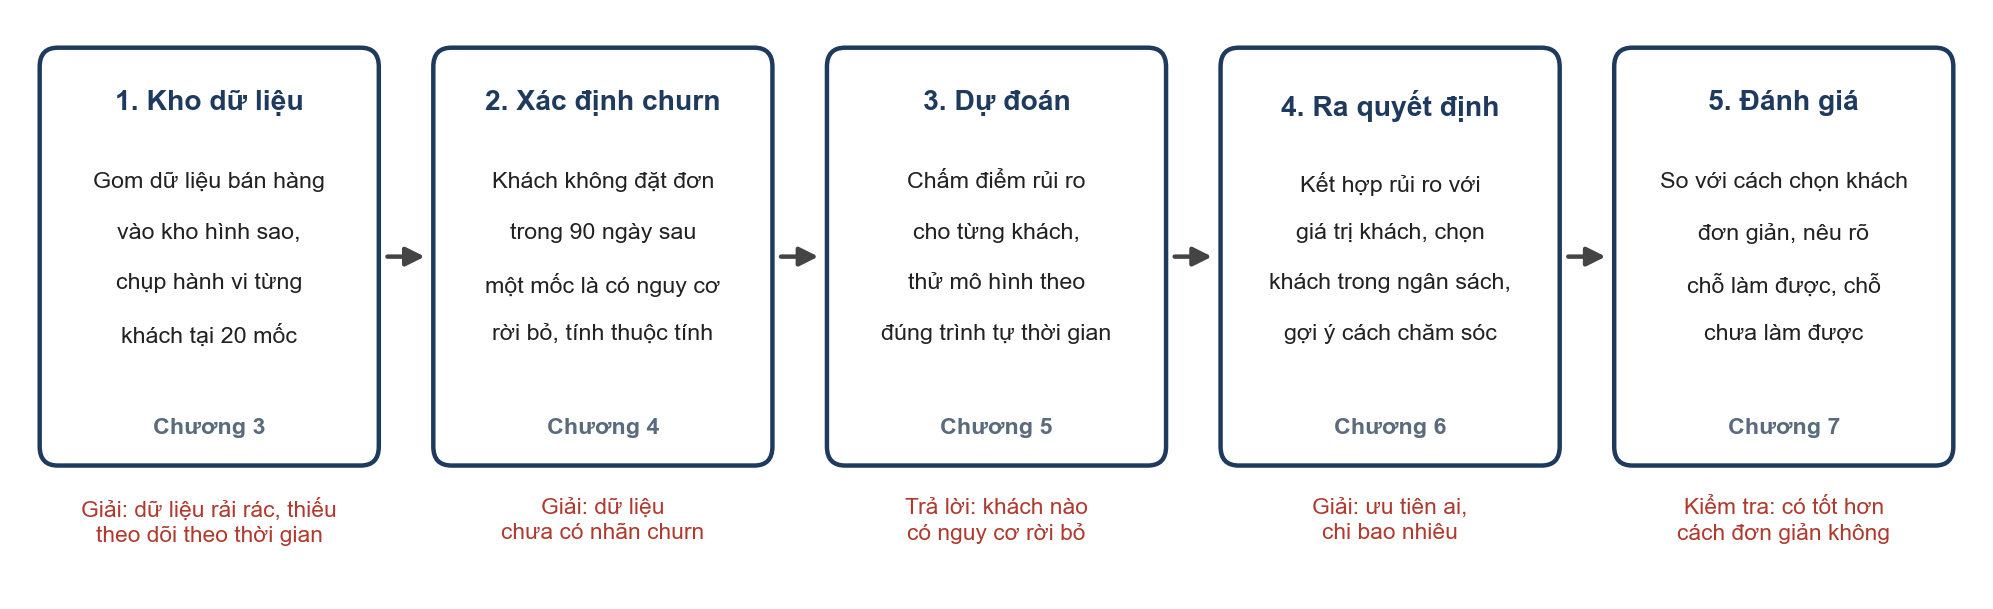
\includegraphics[width=\textwidth]{huong_tiep_can.png}
\caption{Năm bước giải bài toán churn và chương trình bày từng bước}
\label{fig:huongtiepcan}
\end{figure}

Bảng~\ref{tab:giaithachthuc} cho biết bốn thách thức nêu ở mục 1.1 được giải ở đâu.

\begin{table}[!htbp]
\centering
\caption{Bốn thách thức của bài toán churn và cách giải}
\label{tab:giaithachthuc}
\footnotesize
\begin{tabular}{p{3.9cm}p{8.1cm}p{2.5cm}}
\toprule
Thách thức & Cách giải & Trình bày ở \\
\midrule
Dữ liệu chưa có nhãn churn & Tự đặt luật: khách không đặt đơn nào trong 90 ngày sau một mốc thì có nguy cơ rời bỏ & Chương 4 \\
Số liệu tại một thời điểm không cho thấy xu hướng & Bảng Snapshot chụp hành vi từng khách tại 20 mốc, rồi chia khách thành nhóm theo hành vi & Chương 3 và 6 \\
Dữ liệu rải rác, lẫn khách đại lý & Kho dữ liệu hình sao, quy trình ETL, chỉ giữ khách cá nhân và kiểm tra chất lượng & Chương 3 \\
Biết nguy cơ chưa đủ để chọn ai & Hệ hỗ trợ ra quyết định kết hợp rủi ro với giá trị khách, chọn khách trong ngân sách và thử các giả định (what-if) & Chương 6 \\
\bottomrule
\end{tabular}
\end{table}

\subsection{Phạm vi nghiên cứu}
\begin{itemize}
    \item \textbf{Đối tượng:} 18.484 khách hàng cá nhân, toàn bộ mua qua kênh trực tuyến. Nhóm đại lý bị loại vì họ mua theo chu kỳ nhập hàng B2B, khác hẳn hành vi của người tiêu dùng.
    \item \textbf{Dữ liệu:} đơn hàng từ 31/05/2011 đến 30/06/2014. Lịch sử được chia thành giai đoạn quan sát và giai đoạn kiểm tra mua lại, nhờ đó mô hình được kiểm định theo đúng trình tự thời gian.
    \item \textbf{Phân tích:} dựa trên ba đặc trưng hành vi Recency, Frequency và Monetary (RFM). Ba đặc trưng này tóm tắt được hành vi mua chỉ từ dữ liệu giao dịch, vốn là nguồn dữ liệu duy nhất doanh nghiệp có.
    \item \textbf{Công nghệ:} SQL Server và T-SQL cho kho và quy trình ETL, để nguồn và kho cùng một nền tảng. Python (pandas, scikit-learn) cho mô hình, Streamlit cho giao diện DSS.
    \item \textbf{Ranh giới:} hệ thống xếp hạng khách hàng và đề xuất phân bổ ngân sách, không tự gửi tin nhắn đến khách. Hiệu quả giữ chân thực tế chỉ đánh giá được sau khi triển khai.
\end{itemize}

\subsection{Mô tả tập dữ liệu}
Cơ sở dữ liệu tác nghiệp \texttt{CompanyX} có 72 bảng thuộc 6 schema. Dữ liệu đơn hàng trải dài 37 tháng, gồm 31.465 đơn và 121.317 dòng chi tiết, với tổng giá trị thanh toán 123,16 triệu USD. Bảng \texttt{Customer} có 19.820 bản ghi, trong đó 701 bản ghi chưa có đơn nào. Đề tài chỉ dùng 9 bảng liên quan đến hành vi mua, được mô tả trong Bảng~\ref{tab:bang_nguon}.

\begin{table}[!htbp]
\centering\small
\caption{Các bảng nguồn được sử dụng trong đề tài}
\label{tab:bang_nguon}
\begin{tabular}{lrp{6.6cm}}
\toprule
\textbf{Bảng nguồn} & \textbf{Số dòng} & \textbf{Nội dung} \\
\midrule
\texttt{Sales.SalesOrderHeader} & 31.465 & Thông tin chung của đơn hàng: khách hàng, ngày đặt, ngày giao, trạng thái, tổng tiền \\
\texttt{Sales.SalesOrderDetail} & 121.317 & Chi tiết từng sản phẩm trong đơn: số lượng, đơn giá, chiết khấu \\
\texttt{Sales.Customer} & 19.820 & Danh sách khách hàng, phân biệt khách cá nhân và cửa hàng \\
\texttt{Person.Person} & 19.972 & Họ tên của khách hàng cá nhân \\
\texttt{Sales.SalesTerritory} & 10 & Khu vực bán hàng và nhóm quốc gia \\
\texttt{Sales.SpecialOffer} & 16 & Chương trình khuyến mãi áp dụng cho dòng đơn \\
\texttt{Production.Product} & 504 & Danh mục sản phẩm \\
\texttt{Production.ProductSubcategory} & 37 & Tiểu loại sản phẩm \\
\texttt{Production.ProductCategory} & 4 & Loại sản phẩm: Bikes, Components, Clothing, Accessories \\
\bottomrule
\end{tabular}
\end{table}

Dữ liệu có hai giới hạn. Thứ nhất, không có nhãn churn, nên nhãn được suy ra bằng luật 90 ngày ở mục tiêu nghiên cứu. Thứ hai, không có dữ liệu chăm sóc khách hàng (CRM) hay lịch sử chiến dịch. Vì vậy tỷ lệ khách quay lại nhờ chăm sóc và chi phí mỗi lần liên hệ là tham số giả định, người quản lý có thể chỉnh trên giao diện DSS.
